%%%%%%%%%%%%%%%%%%%%%%%%%%%%%%%%%%%%%%%%%%%%%%%%%%%%%%%%%%%%%%%%%
% Dissertacao de Mestrado / Dept Fisica, CFM, UFSC              %
% Andre@UFSC - 2011                                             %
%%%%%%%%%%%%%%%%%%%%%%%%%%%%%%%%%%%%%%%%%%%%%%%%%%%%%%%%%%%%%%%%%

%:::::::::::::::::::::::::::::::::::::::::::::::::::::::::::::::%
%                                                               %
%                          Capítulo 1                           %
%                                                               %
%:::::::::::::::::::::::::::::::::::::::::::::::::::::::::::::::%

%***************************************************************%
%                                                               %
%                         Introdução                            %
%                                                               %
%***************************************************************%

\chapter{Introdução}
\label{sec:Intro}

%***************************************************************%
%                                                               %
%                     Introdução - Nova era                     %
%                                                               %
%***************************************************************%

\section{A nova era da astronomia}
\label{sec:Intro:NovaEra}

Os primeiros {\em surveys}\footnote{Um {\em survey} astronômico é um
levantamento de informações ou mapeamento de regiões do céu utilizando
telescópios e detetores.} espectroscópicos da astronomia extragalática começaram
a ser feitos de forma sistemática na década de 80 \citep{Huchra1988}. Foram
observadas cerca de $2400$ galáxias pelo {\em Center for Astrophysics} em
Harvard \citep{Huchra1983} e aproximadamente $2000$ galáxias pelo {\em Southern
Redshift Survey} \citep{DaCosta1988}. Estes {\em surveys} pioneiros, assim como
alguns dos atuais, visavam primariamente medir {\em redshifts} para estudos da
estrutura em larga escala do Universo.

Nos últimos anos, com o advento dos {\em mega-surveys}, está ocorrendo uma
revolução na forma de fazer ciência na astronomia. Os diversos {\em surveys} em
execução atualmente estão produzindo dados a uma taxa da ordem de petabytes por
ano. Este talvez seja o primeiro campo da ciência onde as informações coletadas
por máquinas tenham -- nas próximas décadas -- um volume maior do que os seres
humanos são capazes de digerir. Uma espécie de {\em Singularidade
Tecnológica}\footnote{O termo {\em Singularidade Tecnológica} se refere a um
futuro hipotético onde uma inteligência superior à humana emerge através da
tecnologia. Qualquer previsão após tal fato se torna muito difícil, algo similar
a um horizonte de eventos, dada a dificuldade em entender uma inteligência
superior à humana.} da astrofísica, onde máquinas coletam, analisam e
classificam dados. O papel do cientista num cenário como este ainda não está
muito claro \citep{Norris2010}.

\subsection{Megalevantamentos de dados}

O {\em Sloan Digital Sky Survey} \citep[\SDSS; ][]{York2000} é referência quando
falamos em {\em surveys} modernos. Em seus $8$ anos de funcionamento, obteve
imagens em $5$ filtros (ver Figura \ref{fig:GalexFilters}) de um quarto do céu e
espectros de um milhão de galáxias. O seu catálogo contém $4$ terabytes de dados
fotométricos e espectroscópicos, e $12$ terabytes de imagens. O \SDSS foi
praticamente o primeiro {\em survey} a conseguir popularizar o acesso aos seus
dados. Estes foram feitos públicos desde o princípio, iniciando uma ``corrida do
ouro'' no seu vasto volume de dados. Esta filosofia é compartilhada hoje pela
grande maioria dos {\em surveys} de grande porte.

Outros {\em surveys} pioneiros nesta era de mega-levantamentos são o
{\em 2dF Galaxy Redshift Survey} \citep[2dFGRS;][]{Colless1999} e o {\em Two
Micron All Sky Survey} \citep[2MASS;][]{Skrutskie2006}. Embora estes {\em
surveys} já tenham sido concluídos, os seus dados permanecem disponíveis
publicamente. Outro exemplo é o arquivo do {\em Hubble Space Telescope}, onde,
embora não sendo um {\em survey} estritamente falando, todas as observações são
disponibilizadas após um ano.

Existem diversos {\em surveys} em operação atualmente. O {\em Wide-field
Infrared Survey Explorer} (WISE) é um telescópio espacial da NASA\footnote{{\em
NASA Explorer Mission} - \url{http://explorers.gsfc.nasa.gov/missions.html}} que
está mapeando o céu inteiro nas faixas de $3,4$, $4,6$, $12$ e
$22\,\mu\mathrm{m}$ do infravermelho \citep{Wright2010}. O {\em Visible and
Infrared Survey Telescope for Astronomy} (VISTA) é um telescópio no Chile
fazendo um {\em survey} do céu do hemisfério sul no infravermelho próximo
\citep{Born2010}. O {\em Kepler} é um telescópio espacial da NASA
\citep{Borucki2010}, semelhante ao WISE, e está fazendo um {\em survey} de uma
região da Via Láctea para descobrir a fração de estrelas com planetas similares
à Terra na nossa Galáxia. Tratado com mais detalhes no capítulo \ref{sec:Galex},
o {\em Galaxy Evolution Explorer} (\galex) está mapeando o céu em ultravioleta.

O projeto J-PAS ({\em Javalambre Physics of the Accelerating Universe
Astrophysical Survey}) é um {\em survey} que pretende imagear um quinto do céu
em $56$ cores \citep{Benitez2009}. Os filtros, de banda estreita, irão cobrir
toda a região óptica, formando um espectro de baixa resolução para cada pixel do {\em
survey}. Serão mais de $200$ terabytes de dados brutos (imagens). O projeto é
uma colaboração entre Espanha e Brasil, com mais de 70 pesquisadores e engenheiros
envolvidos, incluindo integrantes do Grupo de Astrofísica da UFSC. O objetivo do
{\em survey} é a exploração das causas da aceleração do universo, relacionadas à
energia escura. Entretanto, uma quantidade considerável de ciência adicional
poderá ser feita com base no espectro de uma região tão ampla do céu. Seu início
está previsto para 2013.

O LSST ({\em Large Synoptic Survey Telecope}) mapeará metade do céu a cada mês,
aproximadamente, durante cerca de dez anos \citep{Ivezic2008}. Com este
``filme'', em seis bandas espectrais similares às do \SDSS, espera-se fazer um
inventário do objetos do Sistema Solar e explorar os eventos transientes como
Novas, núcleos ativos de galáxias, surtos de raios gama, para citar alguns
exemplos. Este {\em survey} também pretende explorar a natureza da energia
escura, embora, da mesma forma que o J-PAS, os dados possam ser aproveitados
para diversos outros fins. As suas operações científicas têm início previsto
para 2020. Serão mais de um petabyte em imagens brutas por ano, muito mais do
que poderia ser revisado por humanos.

\subsection{Mineração de dados}

Tradicionalmente astrônomos armazenam seus dados em arquivos texto ou binários
contendo um registro por linha, de uma forma tecnicamente conhecida como {\em
flat file}. Buscas neste tipo de banco de dados são feitas examinando
individualmente cada registro do arquivo. Com o volume de dados obtido, por
exemplo, pelo \SDSS ou pelo \galex (aproximadamente $222$ milhões de objetos,
$34$ mil campos), o uso de arquivos simples para armazenamento de dados se torna
inviável. É preciso ``profissionalizar'' o gerenciamento de dados de um {\em
survey} desta escala e aprender a trabalhar com volumes imensos de dados
\citep{Bell2006}.

Técnicas de detecção de padrões em grandes conjuntos de dados, conhecidas como
{\em Mineração de dados}, tiveram um interesse crescente nos últimos anos
\citep{SIGKDD2011}. Estas técnicas têm naturalmente um caráter interdisciplinar,
indo desde aplicações científicas até áreas como Economia \citep{Spanos2000} e
Inteligência de Mercado\footnote{Ferramentas como OLAP ({\em On-line Analytical
Processing}) são usadas por empresas para avaliação de mercado e tomada de
decisão, agindo sobre um grande volume de dados.}.

A equipe de arquivamento do \SDSS desenvolveu uma ferramenta chamada {\em
CasJobs} (ver Seção \ref{sec:CrossMatch:SDSS:CasJobs}), que permite que
múltiplos usuários possam fazer buscas e coleta de dados em seu banco de dados.
Embora o {\em CasJobs} não seja, estritamente falando, uma ferramenta de
mineração de dados, ele facilita, e muito, o acesso aos dados de um {\em
survey}. O presente trabalho se baseia fortemente no uso desta ferramenta.


%***************************************************************%
%                                                               %
%                     Introdução - STARLIGHT                    %
%                                                               %
%***************************************************************%

\section{O catálogo de propriedades físicas do \STARLIGHT}
\label{sec:Intro:Starlight}

O \starlight é um código de síntese espectral desenvolvido por
\citet{CidFernandes2005}. Dado um espectro de galáxia, o programa retorna as
frações de massa e luz correspondentes às populações estelares componentes desta
galáxia. O \starlight expressa o espectro desta galáxia como uma combinação
linear de espectros de populações estelares simples\footnote{Uma SSP consiste
num conjunto de estrelas formadas ao mesmo tempo com a mesma metalicidade.}
(SSP, do inglês {\em Simple Stellar Population}) com diferentes idades e
metalicidades. Matematicamente isto é equivalente a encontrar as componentes do
vetor espectro da galáxia numa base de espectros de SSP, ou seja,
\begin{equation*}
F_\lambda = \sum_{i=1}^{N_\star} x_i F^\star_\lambda(t_i,Z_i)
g_\lambda(A_{V,i}).
\end{equation*}
Nesta equação, $F_\lambda$ é o fluxo em cada comprimento de onda. Os $N_\star$
espectros de base $F^\star_\lambda(t_i, Z_i)$, com $t_i$ e $Z_i$ representando
respectivamente a idade e a metalicidade do elemento de base, são somados com
pesos $x_i$. O conjunto $\{x_i, i=1,2,\ldots,N_\star\}$ é chamado {\em vetor de
população} para a galáxia considerada. O termo $g_\lambda$ corrige o espectro
pelo efeito de atenuação interestelar. Os espectros da base provêm de modelos de
síntese evolutiva de populações estelares. A maior parte dos resultados
publicados do \starlight usa os modelos de \citet[BC03]{Bruzual2003}, do quais
foram extraídas SSPs cobrindo uma ampla gama de idades e metalicidades. São ao
todo 150 SSP diferentes (25 idades e 6 metalicidades) utilizadas na base. O
problema torna-se então um ajuste num espaço de parâmetros bastante grande. A
Figura \ref{fig:StarlightSpectrumSample} mostra o ajuste feito para uma galáxia
do \SDSS.

\begin{figure}
	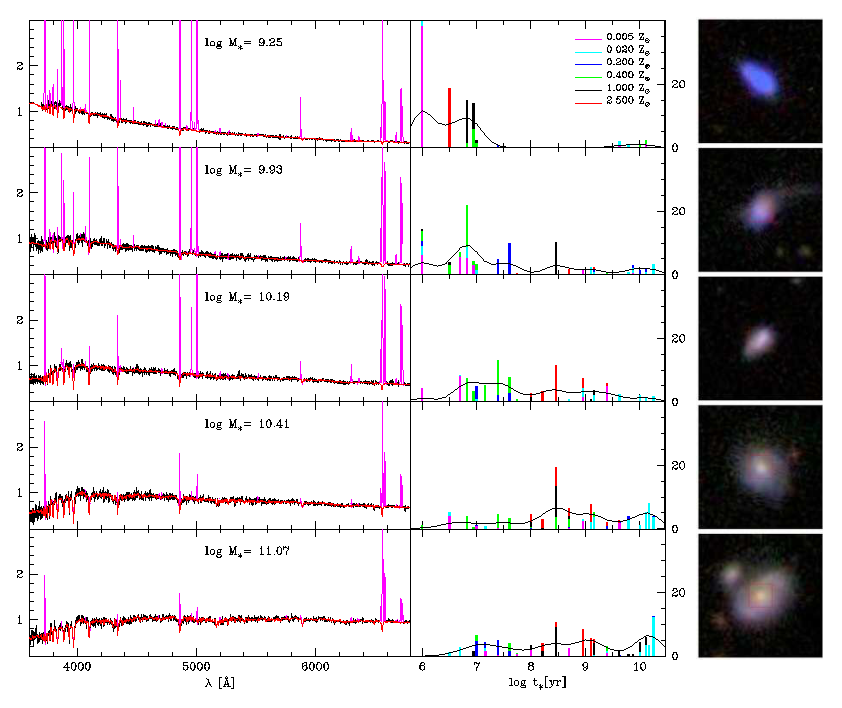
\includegraphics[width=1.0\textwidth]{figuras/starlight-fit.eps}
	\caption[Exemplos de ajuste de espectro com o \starlight.]
	{Exemplos de ajuste de espectros de galáxias com o \starlight
	\citep{Asari2007}. À esquerda, espectros observados (preto), espectros
	modelados (vermelho), com regiões mascaradas em magenta. No meio, a fração da
	luz associada à cada uma das 25 idades das SSPs usadas na síntese, com a curva
	representando a versão suavizada do histórico de formação estelar. À direita,
	imagens do \SDSS correspondentes às galáxias.}
	\label{fig:StarlightSpectrumSample}
\end{figure}

Analisando o vetor de população das galáxias é possível obter algumas de suas
propriedades físicas. É possível também extrair as medidas das linhas de emissão
-- não modeladas no ajuste -- com bastante precisão. A técnica foi aplicada aos
espectros de galáxias do \SDSS e o resultado da síntese gerou um catálogo de
propriedades físicas e linhas de emissão de quase um milhão de galáxias.
Disponibilizado em \url{http://www.starlight.ufsc.br/}, este banco de dados já
foi utilizado por dezenas de pesquisadores em todo o mundo, resultando em vários
artigos \citep[para citar alguns]{Bian2006, Liang2007, Peeples2009,
Lara-Lopez2009, Lara-Lopez2010} e teses \citep{Mateus2006, Gomes2009,
Asari2010}.


%***************************************************************%
%                                                               %
%                 Introdução - Este trabalho                    %
%                                                               %
%***************************************************************%

\section{Este trabalho}
\label{sec:Intro:EsteTrab}

Historicamente a região ultravioleta (UV) do espectro eletromagnético tem sido
pouco estudada na astronomia. Não por falta de interesse dos astrônomos, mas
pelo simples fato de que observações feitas de dentro da atmosfera são
impossibilitadas pela camada de ozônio. É preciso ir para o espaço. Foram
lançados diversos satélites com o intuito de estudar o céu em UV (ver Seção
\ref{sec:Galex:CeuUV}). O \galex foi o primeiro telescópio espacial a fazer um
{\em survey} do céu inteiro em UV. A missão tem como objetivo estudar a evolução
da taxa de formação estelar em galáxias \citep{Martin2005}.

Embora este e outros grandes {\em surveys} tenham um grande valor
individualmente, esta é somente a ponta do {\em iceberg}. Cruzando informações
de {\em surveys} em diversos comprimentos de onda pode-se ter uma nova percepção
da relação entre os processos físicos subjacentes. Este trabalho utiliza dados
obtidos dos {\em surveys} \SDSS e \galex, nas bandas espectrais óptica e UV,
respectivamente. Estes dois {\em surveys} foram indexados (ver Seção
\ref{sec:Crossmatch:SDSSGalex}) de forma a facilitar a identificação entre as
suas detecções. A técnica desenvolvida por eles pode ser aplicada em
virtualmente qualquer outro {\em survey} astronômico.

As galáxias utilizadas na síntese do \starlight foram obtidas do catálogo do
\SDSS. Neste trabalho foi feita a identificação destas galáxias no catálogo do
\galex, obtendo-se assim as suas medidas de fotometria UV. Este conjunto de
dados formou uma amostra de galáxias com as suas propriedades físicas, cores
ópticas e cores UV. As galáxias desta amostra são classificadas utilizando o
diagrama de diagnóstico WHAN, conforme \citet{CidFernandes2011}. Este método de
classificação utiliza as linhas de emissão \Halpha e \NII para separar as
galáxias nas classes de formação estelar, núcleo ativo, ``aposentadas'' e
passivas. As cores UV das galáxias de cada classe são analisadas em busca de
correlações e tendências.

\subsection{Organização deste trabalho}

No capítulo seguinte, a missão \galex é tratada em mais detalhes. As
características do {\em survey} são discutidas e são apresentados alguns
resultados importantes. Os produtos gerados pelos {\em surveys} do \galex e o
acesso a estes dados são descritos no final do capítulo.

O terceiro capítulo introduz o uso de bancos de dados em astronomia. Em seguida
é tratado o problema genérico de identificação cruzada ({\em crossmatch}) de
objetos em catálogos de {\em surveys} astronômicos. Os bancos de dados do \SDSS
e do \starlight são apresentados, e o processo de {\em crossmatch} é feito entre
os catálogos do \SDSS e do \galex. Finalmente, define-se uma amostra com
magnitudes absolutas (ópticas e UV) e propriedades físicas das galáxias.

No quarto capítulo é feita a análise da amostra obtida no capítulo anterior. As
galáxias são classificadas através do diagrama WHAN, introduzido por
\citet{CidFernandes2010, CidFernandes2011}, e as propriedades físicas destas
galáxias (obtidas do \starlight) são analisadas de acordo com as suas cores
ópticas e UV.

No quinto e último capítulo são apresentadas as conclusões e perspectivas deste
trabalho.

As {\em queries} SQL utilizadas neste trabalho estão listadas no apêndice
\ref{apendice:Queries}.

% End of this chapter
